\documentclass[a4paper,12pt]{report}
\usepackage{listings}
\usepackage[utf8]{inputenc}
\usepackage{import}
\usepackage[utf8]{inputenc}
\usepackage{textcomp}
\usepackage{float}
\usepackage{subfig}
\usepackage{mathtools}
\usepackage{setspace}
\usepackage{graphicx}
\usepackage{graphics}
\usepackage{epstopdf}
\usepackage[toc,page]{appendix}
\usepackage{parskip}
\usepackage{enumerate}


%\usepackage[spanish,es-tabla]{babel}
%\usepackage[nottoc,numbib]{tocbibind}
\renewcommand{\baselinestretch}{1.5}
%caracteristicas de paginas
\pdfpagewidth 8.3in
\pdfpageheight 11.7in
\setlength\oddsidemargin{-0,21in}
\setlength\evensidemargin{-0,21in}
\setlength\topmargin{-2cm}
\setlength\textwidth{6.50in}
\setlength\textheight{23.7cm}
\setlength\parskip{0.1in}
\def\thechapter{\arabic{chapter}}
\newcommand{\forceindent}{\leavevmode{\parindent=1em\indent}}

\renewcommand{\chaptername}{Capítulo}
\renewcommand{\contentsname}{Contenidos}
\renewcommand\bibname{Bibliografía}
\renewcommand\appendixname{Apéndice}
\renewcommand\appendixpagename{Apéndices}
\addappheadtotoc
\renewcommand\appendixtocname{Apéndices}

% Biblio: http://www.csse.monash.edu.au/documents/bibtex/

\begin{document} 

\thispagestyle{empty}

\begin{center}

% Parte Superior
 \begin{figure}[htb]
\centering
\includegraphics[width=0.45\textwidth]{caratula/logo.png}
\end{figure} 



\textsc{\LARGE Universidad de Buenos Aires}\\[0.5cm]
\textsc{\large Facultad de Ciencias Exactas y Naturales}\\[0.5cm]

\textsc{  Departamento de Física Juan José Giambiagi}\\[0.5cm]


% Titulo
%\HRule \\[0.4cm]
\huge Título de la tesis\\
%\HRule \\[1cm]

\textsc{\large Tesis de Licenciatura}\\[1cm]

% Autores y Directores
{\LARGE \textbf{
Ignacio Mariano Sticco}} \\ [1cm]

\large
Director: Dr. Claudio Oscar Dorso \\[0.5cm]
Codirector: Dr. Guillermo Alberto Frank
\vfill

% Parte Inferior

 Agosto de 2016

\end{center}

\newpage


\begin{flushleft}
TEMA: Título de la tesis\\

ALUMNO: Ignacio Mariano Sticco\\

LU N$^{\circ}$: 888/10 \\

LUGAR DE TRABAJO: Instituto de Astronom\'ia y F\'isica del Espacio, Consejo Nacional de Investigaciones Cient\'ificas y T\'ecnicas (CONICET) - Universidad de Buenos Aires (UBA)\\

DIRECTOR DEL TRABAJO: Dr. Claudio Oscar Dorso \\

CODIRECTOR DEL TRABAJO: Dr. Guillermo Alberto Frank\\

FECHA DE INICIACI\'ON: Septiembre de 2015 \\

FECHA DE FINALIZACI\'ON: Agosto de 2016\\

FECHA DE EXAMEN:  \\

INFORME FINAL APROBADO POR:
\end{flushleft}                                                              %
                                                            %
\vspace{2cm}

\begin{center}
\begin{tabular}{|c|c|}
\hline
Autor &  \,\,\,\,\, \,\,\,\,\,\,\,\,\, \,\,\,\,\,\,\,\,\,\,\,\,\,\,\,\,\,\,Jurado \,\,\,\,\,\,\,\,\,\,\,\,\,\,\,\,\,\,\,\, \,\,\,\,\,\,\,\,\,\,\,\, \\
&            \\
       &            \\
  ..............................            &     ..............................          \\
       &            \\

\hline
Director &      \,\,\,\,\, \,\,\,\,\,\,\,\,\, \,\,\,\,\,\,\,\,\,\,\,\,\,\,\,\,\,\,Jurado \,\,\,\,\, \,\,\,\,\,\,\,\,\,\,\,\,\,\,\,\,\,\,\,\, \,\,\,\,\,\,\,\\
&            \\
       &            \\
  ..............................            &       ..............................        \\
         &            \\
 \hline
Profesor de Tesis de Licenciatura &  \,\,\,\,\,\,\, \,\,\,\,\, \,\,\,\,\,\,\,\,\,\,\,\,\,\,\,\,\,\,\,\,Jurado \,\,\,\,\,\,\,\,\,\,\,\,\,\,\,\,\,\,\,\,\,\,\,\,\,\,\, \,\,\,\,\,\\
&            \\
       &            \\
  ..............................            &      ..............................         \\
         &            \\
\hline
\end{tabular}
\end{center}

%\section*{}
%A mi codirector Guillermo Frank que con su vocación docente supo enseñarme las bases de la física computacional y contagiarme el entusiasmo por la labor del día a día. \\

A mi director Claudio Dorso que gracias a ese balance entre buen humor y exigencia logra que las cosas funcionen como deben. \\

A Pablo Alcaín, embajador de la buena programación, brindó muchísimo apoyo en esta investigación, sus consejos siempre van en la dirección correcta. \\

A Fernando Cornes, Guillermo Pascualetti y Sebastián Pinto, con quienes compartí almuerzos, espacio de trabajo e información valiosa. 

A mi papá y mi mamá que fomentan mi bienestar de innumerables maneras. A mi hermana Magui por sus charlas amenas y profundas a la vez. A mi hermano Patri, su colaboración fue clave para avanzar con algunos asuntos computacionales.\\

A mi abuela Ada, por todos esos almuerzos tan cargados de alegría como de comida deliciosa. A mi tía Meme quien me dio ánimos en momentos de desgano.\\

A mi abuelo Abel, siempre estimuló mi curiosidad y mucho tuvo que ver con mi incursión en la ciencia. \\

A mis amigos Hernan Martinelli e Ignacio Sallaberry, juntos desde el comienzo de la carrera. Por todos esos encuentros catárticos acompañadas de cerveza.\\ 

A mi amor Ana Rosso, compañera de charlas nerd, caminatas relajantes e infinitos momentos llenos de risas. Sin ella no tendría la paz que necesito para estar bien. 
\tableofcontents
\chapter{Introducción}
\section{Antecedentes}

La práctica de incluir dos puertas para evacuaciones de emergencia se remonta a los tiempos de la última dinastía Qing en China (1644-1911 AD). Existía una ley que establecía que los edificios grandes debían tener dos salidas para evitar problemas en caso de incendio~\cite{cheng}.
Los códigos estándar actuales cuantan con especificaciones detalladas de las ubicaciones de las puertas, el ancho y la separación entre éstas~\cite{OSHA,FLO}.
 
Las reglamentaciones actuales exigen que el ancho mínimo de las puertas debe ser 0,813~m y el tamaño máximo de una hoja no debe ser mayor a 1,219~m\cite{FLO,FLO2}. Si se requieren más de dos puertas, la separación entre dos de ellas debe ser al menos un cuarto o un tercio de la distancia diagonal de la habitación. No hay ningún requerimiento especial sobre el resto de las puertas, más alla del hecho que no deben estar simultaneamente bloqueadas\cite{FLO,FLO2}.\\

La reglamentación da lugar a ubicar las salidas adicionales (\emph{i.e.} las puertas arriba mencionadas) con una distancia de separación arbitraria. De esta forma, se pueden ubicar dos puertas en un mismo flanco del cuarto. El caso especial de dos puertas contiguas ha sido examinado en la literatura~\cite{kirchner1,perez1,daoliang1,huanhuan1}. \\

Kirchner y Schadschneider estudiaron el proceso de evacuación de peatones a través de dos puertas contiguas usando un modelo de autómatas celulares\cite{kirchner1}. Los agentes podían abandonar la habitación con comportamientos que iban desde el individualismo hasta un movimiento fuertemente acoplado como el de una \emph{manada}. Se encontró que el tiempo de evacuación es independiente de la distancia de separacipón para el caso de peatones con comportamiento individualista. Pero, si los peatones se movían en manada, se reportó un tiempo de evacuación mayor para pequeñas separaciones (menores al tamaño de 10 individuos).\\

El número de peatones que abandonó el recinto por unidad de tiempo mostró una disminución para distancias de separación menores al ancho de cuatro puertas\cite{perez1}. Esta disminución del flujo fue asociada a un efecto de interferencia debido a peatones cruzandose mutuamente. El umbral de cuatro anchos de puerta ($4\,d_w$) corresponde a la distancia de separación necesaria para distinguir dos  grupos independientes de peatones, cada uno de ellos rodeando a la puerta más cercana. \\

Los investigadores destacaron el hecho que no importa cuan separadas estén las dos puertas, el rendimiento de la evacuación no mejora el doble respecto al rendimiento que tiene una única salida (con el mismo ancho). Este efecto se le atribuye a algún tipo de interferencia entre peatones\cite{perez1}.\\

Aunque los resultados arriba mencionados fueron obtenidos para puertas muy angostas (\emph{i.e.} del ancho de un individuo), investigaciones posteriores mostraron que también aplican a puertas que permiten el paso de dos peatones. Sin embargo, esto no aplica a habitaciones con una única puerta\cite{daoliang1}. En este caso, el flujo medio de peatones evacuados aumenta con el ancho de la puerta, pero el flujo por unidad de ancho decrese\cite{daoliang1}. \\
 
El rendimiento de la evacuación puede verse afectado por la distancia de separación de las puertas si éstas estan ubicadas cerca de una pared, es decir, cerca de la esquina del cuarto. La gente entra en contacto con las paredes, perdiendo eficiencia en la evacuación\cite{kirchner1,daoliang1}. \\

Investigaciones más detalladas con automatas celulares mostraron que el rendimiento en la evacuación depende de cinco longitudes: el ancho total de las salida (es decir, sumar los anchos de cada puerta), la distancia de separación entre puertas, la diferencia de ancho entre las puertas y la distancia a la esquina más cercana \cite{huanhuan1}. \\

El ancho total de las salidas puede mejorar el tiempo de evacuación para cualquier distancia de separación entre puertas, siempre que ambas tengan el mismo ancho. 
Sin embargo, la separación controla la ubicación óptima para
estas salidas. A grandes rasgos, la distancia de separación $d_g$ debe ser igual a $L-4\,d_w$, donde $L$ es la longitud del cuarto\cite{huanhuan1}. \\

La ubicación optima concuerda con el fenómeno de disminución del flujo para pequeños valores de $d_g$. También se condice con el empeoramiento del rendimiento de la evacuación para puertas cercanas a la esquina. Pero esta disminución puede surgir por otras razones, ya que el aumento del recorrido de los peatones a las puertas juega un papel importante.\\ 

La configuración con dos puertas no necesita ser simétrica a lo largo de la pared. La asimetría provoca demoras que dependen de la diferencia del ancho de las puertas y sus posiciones relativas. Ubicar a la puerta más ancha en el medio de la pared y a la menor en la esquina, ocasiona un mejora en el proceso de evacuación\cite{huanhuan1}.\\

Esta investigación se centra en configuraciones simétricas con puertas de igual tamaño. A diferencia de la literatura arriba mencionada, se examina la dinámica de la evacuación a través del modelo de fuerza social. En el capítulo siguiente se encuentra una descripción de este modelo. \\

\section{Objetivos}

\chapter{Marco Teórico}
En este capítulo se describirá el modelo en el cual se basa toda la investigación, también se definirán los conceptos utilizados a lo largo del trabajo como la definición de la presión social y los blocking clusters. Además se comentará el algoritmo de Verlet, ya que fue utilizado para resolver la dinámica del problema. 

\section{Modelo de Fuerza social}

El modelo de fuerza social es un modelo basado en agentes utilizado para simular el movimiento de peatones. Supone que los individuos soportan tres tipos de fuerzas: fuerzas de deseo (autopropulsión), sociales (repulsión) y granulares (rozamiento).  \\

La fuerza de autopropulsión refleja el hecho que el individuo i-esimo que poseé masa $m_i$, desea  moverse con una velocidad $v_d^ {(i)}(t)$ en una dirección $\hat{\mathbf{e}}_d^ {(i)}(t)$, por lo tanto readapta su velocidad $\mathbf{v}_i(t)$ con un cierto tiempo característico $\tau$.
\begin{equation}
\mathbf{f}_d^ {(i)}(t)=m_i\,\displaystyle\frac{v_d^ {(i)}(t)\,\hat{\mathbf{e}}_d^ {(i)}(t)-\mathbf{v}_i(t)}{\tau}\label{fdeseo}
\end{equation}

La repulsión social es una fuerza que describe la tendencia que tienen las personas a mantenerse alejadas unas de otras. Depende de la distancia de separación entre individuos $d_{ij}=\left\|\mathbf{r_i}-\mathbf{r_j}\right\|$ y está en la dirección normal $\mathbf{n}_{ij}=(n_{ij}^1,n_{ij}^2)/d_{ij}$ (versor que apunta desde el individuo j al individuo i). Los peatones están en contacto si el valor de $d_{ij}$ es más chico que la suma de los radios $r_{ij}=(r_i+r_j)$. $A_i$ y 	$B_i$ son constantes.

\begin{equation}
\mathbf{f}_s^{(ij)}=A_i\,e^{(r_{ij}-d_{ij})/B_i}\mathbf{n}_{ij}\label{fsocial}
\end{equation} 

Cuando los individuos están en contacto, comienza a actuar una fuerza de rozamiento, la misma es proporcional a la velocidad relativa entre individuos.  
$\Delta \mathbf{v}_{ij}=(\mathbf{v}_i-\mathbf{v}_j)$, la dirección tangencia está representada por $\mathbf{t}_{ij}=(-n_{ij}^2,n_{ij}^1)$.  $\kappa$ es una constante y $g(x)$ es una función nula cuando los individuos no se toca $(r_{ij}<d_{ij})$ y toma el valor de su argumento en caso contrario. 
\begin{equation}
\mathbf{f}_g^{(ij)}=\kappa\,g(r_{ij}-d_{ij})\,\Delta \mathbf{v}_{ij}\cdot\mathbf{t}_{ij}\label{frozamiento}
\end{equation}

Se trata de forma análoga a la interacción de los individuos con las paredes. $d_{iW}$ es la distancia del i-esimo peatón con la pared W, $n_{iW}$ la dirección perpendicular entre éstos y $t_{iW}$ la tangencial. La expresión \ref{fparedes} agrupa tanto a la repulsión como al rozamiento de la interacción peatón-pared.

\begin{equation}
\mathbf{f}^{iW}=A_ie^{(r_{i}-d_{iW})/B_i}\mathbf{n}_{iW}-\kappa g(r_{i}-d_{iW})\Delta \mathbf{v}_{i}\cdot\mathbf{t}_{iW}
\label{fparedes}
\end{equation} 

Con todo esto, mediante la fórmula \ref{newton}, puede expresarse el cambio de velocidad en el tiempo que siente un individuo. $f^{ij}$ es el término de interacción entre individuos, es la suma de la repulsión y el rozamiento. El cambio de posición viene dado por $v_{i}(t)=d\mathbf{r_i}/dt$.

\begin{equation}
m_i\frac{d\mathbf{v_i}}{dt}=\mathbf{f}_d^ {(i)}(t)+ \sum_{i\neq j}^{N}\mathbf{f}^{(ij)} + \sum_{W}^{N}\mathbf{f}^{(iW)}
\label{newton}
\end{equation}  
 
\section{Presión social}

\section{Blocking Clusters}

Se utilizó el concepto de blocking cluster para estudiar a los individuos más cercanos a la salida. Se lo define como un conjunto de individuos en contacto que va desde un punto de la pared hacia otro. Estos puntos están proximos a los costados de la puerta. Aquellos peatones que conforman el blocking cluster son los responsables de bloquear la salida.  Tipicamente los blocking cluster formados en las evacuaciones tiene estructura de "arco" como el que se muestra en la figura \ref{bc}. Basta que un solo peaton deje de estar en contacto con sus vecinos para que el blocking cluster deje de estar constituído. \\

\begin{figure}[H]
    \centering
    \includegraphics[height=5.5cm]{figuras/dos_puertas.png}
    \caption[width=5cm]{}
    \label{bc}
\end{figure}

A lo largo del trabajo se han usado dos tipos de blocking clusters: Big blocking cluster y small blocking cluster. El primero se tiene cuando hay dos puertas sobre la misma pared, son los individuos que van desde una puerta hasta la otra (encierran las dos salidas). El segundo es el bloqueo de una única salida. 

\section{Algoritmo de Verlet}

Para integrar las ecuaciones de moviemiento se usó el algoritmo de Verlet. El mismo se basa en actualizar las velocidades, luego las posiciones, en tercer lugar actualiza las fuerzas y vuelve a repetir el ciclo hasta completar las trayectorias. 

%% Poner fórmulas, ventajas y orden del error. (ver haile)


 
\chapter{Simulaciones}

\noindent En este capítulo se describirán los métodos usados para llevar a cabo las simulaciones. 

\noindent Para realizar las simulaciones se utilizó el programa LAMMPS (Large-scale Atomic/Molecular Massively Parallel Simulator).
Es un software de código libre distribuido bajo los términos de GPL.
LAMMPS se caracteriza por hacer uso de las listas de vecinos [rapaport] para efecuar cálculos que permiten reducir la
complejidad algorítmica, además cuenta con una gran cantidad de funciones implementadas orientadas al uso de simulaciones
de dinámica molecular. 

\noindent Todas las simulaciones constaron de N individuos en un recinto cuadrado cuyo tamaño estaba ligado a la cantidad de
peatones de modo tal que mantenga constante la densidad. En una de las paredes se ubicó una o dos puertas dependiendo de qué 
se buscaba analizar.
Para todas los sistemas estudiados se configuró un arreglo bidimensional de individuos, ordenados inicialmente tipo
red cuadrada, separados entre si por una distancia de 1,3 m. La velocidad inicial se estipuló de modo que todos los individuos
tengan en promedio 1.7 m/s (en módulo) con una dispersion de m/s, la dirección fue generada aleatoriamente para
cada uno de ellos. Luego del instante inicial, los agentes cambiaban su velocidad acorde a la velocidad de deseo configurada 
(con el fin de que todos busquen evacuar la habitación). Una vez que los individuos abandonaban el recinto no se los reinyectaba.
De modo que al evacuar dejaba de importar sus observables. 
Para resolver la dinámica se utilizó el algoritmo de Verlet. 
\noindent Con el fin de compatibilizar el modelo de fuerza social con LAMMPS, se crearon varios módulos con las fuerzas que
caracterizan al modelo y algulas fnnciones que sirvieron para caracterizar al sistema. Todos estos fueron escritos en c++.

\section{Módulos}

{\Large pair\_social}

Este módulo se hizo para incluir la fuerza social del modelo de Helbing. Toma como parámetros la constante B y la distancia 
de corte (si los individuos estan separados por una distancia mayor a este corte, la fuerza social entre ellos no se calcula).
Otros parámetros son agregados a través de la función pair\_coef. Estos son la constante A del modelo de Helbing, la distancia 
de corte y el radio de los individuos. Los valores utilizados fueron: A $=$ 2000, B$=$ 0,08 r\_cut $=$ 3,5 d $=$ 0,30.
La elección de la distancia de corte se tomó de modo tal que la fuerza social que sienten individuos separados a esa distancia
sea despreciable ($\sim$ 10$^{-12}$). El resto de los parámetros se extrajeron de la bibliografia del modelo de fuerza social[].

{\Large pair\_gran\_social}

Se creó para que exista rozamiento entre los individuos que están en contacto. Requiere como parámetro el valor de la constante de rozamiento, el mismo fue $\kappa =$ 240000, tanto este valor como la expresión de la fuerza son acordes al modelo de Helbing.

{\Large fix\_wall\_social y fix\_wall\_gran}

Estos módulos son análogos a pair\_social y pair\_gran\_social pero aplicados a las fuerzas de interacción entre los individuos y las paredes. El primero simula la fuerza de repulsión y poseé los mismos parámetros que la repulsión entre individuos mientras que el segundo modela la fuerza de rozamiento dinámico. 

{\Large fix\_social\_self y fix\_social\_self\_multi}

La fuerza de deseo del modelo de Helbing fue simulada con estos módulos. El primero se usó para los recintos con una única puerta mientras que el segundo para recintos con dos. 
El primero requiere como parámetro la masa de los individuos y la velocidad de deseo. El target que tiene cada individuo, depende de la posición en donde se encuentre. Por cada puerta hay tres targets: superior, medio e inferior. El medio está ubicado en la mitad de la puerta, los otros 0,3 m por encima y por debajo.  Los individuos cuya posición en la coordenada 'y' sea mayor (menor) que el target superior (inferior) actualizan su velocidad para apuntar al target superior (inferior). Si se encuentran en medio de éstos, apuntan al centro de la puerta. 
Cuando se simularon recintos con dos puertas se usó fix$\_$social$\_$self$\_$multi, sus parámetros son: la masa de los individuos, la velocidad de deseo y el gap (la distancia de separación entre puertas). Si el gap es nulo, las dos puertas estan unidas (formando una única puerta ancha). En este caso, se establecen tres targets: el superior (inferior) 0.3 m debajo (encima) del final de la puerta superior (inferior). Los individuos que se encuentran en el medio apuntan al centro (al igual que en el caso de una única puerta).
Si el gap es no nulo, es decir, existe una porción de pared entre ambas puertas, la dirección de la velocidad de los individuos se actualiza de forma análoga al caso de una puerta. 

{\Large compute\_social\_pressure}

Calcula la presión que siente cada individuo debida a la interacción de repulsión social. Para cada timestep devuelve un vector con la pesión de cada uno. 

{\Large compute\_dijkstra\_atom}

Rotula con la misma etiqueta a todos los elementos que forman parte de un blocking cluster. Requiere como parámetro las posiciones en la coordenada 'y' de los puntos de origen y terminación del blocking cluster y la posición de la pared en la coordenada 'x'. Para cada timestep, devuelve un vector con un número no nulo para los individuos que forman el cluster de bloqueo y cero para los que no. 

\chapter{Resultados y Discusión}
\label{resultados}

\begin{flushleft}
 {\footnotesize{ \textsl {An intellect which at a certain moment would know all forces that set nature in motion, and all positions of all items of which nature is composed, if this intellect were also vast enough to submit these data to analysis, it would embrace in a single formula the movements of the greatest bodies of the universe and those of the tiniest atom; for such an intellect nothing would be uncertain and the future just like the past would be present before its eyes.}}} \\
\footnotesize  Pierre Simon Laplace, A Philosophical Essay on Probabilities, 1795.\\
\end{flushleft}

En este capítulo se discutirán los resultados obtenidos en el trabajo. Está dividido en dos secciones, la primera está dedicada a recintos con una única puerta y la segunda a recintos con dos puertas sobre la misma pared.  

\section{\label{una_puerta} Una puerta}

En esta sección se estudiará el caso de un recinto cuadrado con 225 individuos y una sola puerta. Se compararán los campos de presión y velocidad para recintos con puerta ancha (3,6~m) y angosta (1,2~m). También se hará una comparación de la presión y velocidad en función del tiempo que posee un individuo que comienza en el medio de la habitación. Se discutirá, además, cómo varía la presión según la distancia a la salida.     

\subsubsection{Puerta ancha (3,6~m)}

Los resultados que se presentan en esta subsección son de simulaciones hechas para un recinto de  $20\times 20$~(m) con 225 individuos y una puerta centrada en la posición $x=20$~m e $y=10$~m con un ancho $L=3,6$~m.\\

En la figura \ref{isobaras_flujo_3_6m} (izquierda) se muestra un gráfico de isobaras. La presión que aparece en estos gráficos fue calculada a partir de la expresión (\ref{phelbing}). Puede verse que la zona de mayor presión se da a los costados de la puerta mientras que en el medio la presión es menor (sobre todo en la zona más próxima a la puerta). La distribución de presiones es simétrica con respecto al eje $y=10$~m.  

\begin{figure}[H]
    \centering
    \includegraphics[scale=1]{figuras/press_225p_v4_onedoor_3_6.eps}
    \hfill
        \includegraphics[scale=1]{figuras/flujo_door_3_6m.eps}
    \caption[width=5cm]{Izquierda: Isobaras cercanas a la puerta; la escala a la derecha está expresada en [P]=N/m. Derecha: Gráfico de flujo de velocidad. Para ambos gráficos, la salida está centrada en la posición $x=20$~m e $y=10$~m y tiene ancho $L=3,6$~m. El recinto es de $20\times 20$~(m) con 225 individuos. La gráfica corresponde a valores medios a lo largo de 30 procesos de evacuación. Se usó un grillado de 1m$^2$ para promediar los campos de presiones y velocidad. La velocidad deseada de los individuos fue de $v_d=4$~m/s. Las barras rojas representan las paredes laterales.}
    \label{isobaras_flujo_3_6m}
\end{figure}

El gráfico de la derecha muestra el promedio del flujo de velocidades. El ancho del trazo denota la magnitud del módulo de la velocidad. La mayor celeridad se obtiene en la zona del medio (en la coordenada $y$), mostrando que los individuos que se encuentran en dicha región evacúan más rápido que los individuos que van por los costados. 
Puede verse que las zonas de alta presión coinciden con zonas de baja velocidad (costados) mientras que las zonas de alta velocidad son áreas con menor presión (centro). \\

La relación entre presión y velocidad se condice con los resultados obtenidos en la figura \ref{pa_vel_t_100_3_6}. Allí se muestran la presión y velocidad en función del tiempo para un individuo que comienza en el medio de la habitación ($x=12,35$~m e $y=8,45$~m). Al principio su velocidad aumenta sin que la presión se vea afectada ya que corre en la zona de baja densidad local (sin interactuar con el resto de los peatones). Luego, su velocidad disminuye conforme su presión se incrementa. En este momento la salida se obstruye y la multitud se amontona. Finalmente la velocidad vuelve a aumentar mientras que su presión disminuye; en este momento el individuo logra hacerse paso para evacuar. 

\begin{figure}[H]
    \centering
    \includegraphics[scale=1.6]{figuras/p_vel_t_100_3_6.eps}
    \caption[width=5cm]{Gráfico de velocidad(inferior) y presión(superior) en función del tiempo para un individuo ubicado inicialmente en $x=12,35$~m e $y=8,45$~m.  La salida está centrada en la posición $x=20$~m e $y=10$~m y tiene ancho $L=3,6$~m. El recinto es de $20\times 20$~(m) con 225 individuos. La gráfica corresponde a dos iteraciones diferentes (variando la velocidad inicial). La velocidad deseada del individuo fue de $v_d=4$~m/s.}
    \label{pa_vel_t_100_3_6}
\end{figure}

En resumen, cuando la puerta es ancha, alta presión implica baja velocidad. Este fenómeno se evidencia tanto en los campos de presión y velocidad como en la evolución temporal de un individuo en particular. 

\subsubsection{Puerta angosta (1,2 m)}

Los resultados que se exhiben en esta subsección corresponden a simulaciones hechas para un recinto de  $20\times 20$~(m) con 225 individuos y una puerta centrada en la posición $x=20$~m e $y=10$~m con un ancho $L=1,2$~m. El tamaño de la puerta angosta coincide con el ancho de hombros de dos individuos.\\

En el gráfico izquierdo de la figura \ref{isobaras_flujo_1_2m} se muestra la distribución de presión para este tipo de recintos. La presión máxima se da en el centro, a diferencia de lo que ocurre en recintos con puerta ancha, donde la máxima presión está a los costados.\\

En el gráfico derecho de la figura \ref{isobaras_flujo_1_2m} se exhibe el flujo de velocidad. Al igual que en la imagen derecha de  \ref{isobaras_flujo_3_6m}, la máxima celeridad se da en el medio (coordenada $y$).
Cabe destacar que la zona de mayor velocidad no coincide con una región de baja presión. De hecho se tiene máxima presión y velocidad en la misma área.  

\begin{figure}[H]
    \centering
    \includegraphics[scale=1]{figuras/fig4_version0.eps}
    \hfill
        \includegraphics[scale=1]{figuras/flujo_door_1_2m.eps}
    \caption[width=5cm]{Izquierda: Isobaras cercanas a la puerta; la escala a la derecha está expresada en [P]=N/m. Derecha: Gráfico de flujo de velocidad. Para ambos gráficos, la salida está centrada en la posición $x=20$~m e $y=10$~m y tiene ancho $L=1,2$~m. El recinto es de $20\times 20$~(m) con 225 individuos. La gráfica corresponde a valores medios a lo largo de 30 procesos de evacuación. Se usó un grillado de 1m$^2$ para promediar los campos de presiones y velocidad. La velocidad deseada de los individuos fue de $v_d=4$~m/s. Las barras rojas representan las paredes laterales.}
    \label{isobaras_flujo_1_2m}
\end{figure}

En la figura \ref{pa_vel_t_100_1_2} se presenta un gráfico de presión y velocidad en función del tiempo para un individuo cuya posición inicial es: $x=12,35$~m e $y=8,45$~m. Luego de los primeros segundos (estado estacionario), los momentos en los que soporta alta presión son momentos de baja velocidad y viceversa. Esto coincide con lo obtenido para un peatón con la misma posición inicial en una habitación con puerta ancha (fig. \ref{pa_vel_t_100_3_6}).A pesar de esta similitud, notar que el individuo tarda mucho más tiempo en evacuar el recinto cuando la puerta es angosta. \\

Puede decirse que para recintos de puerta angosta, en cada instante de tiempo, se mantiene la correlación presión-velocidad (fig \ref{pa_vel_t_100_1_2}); sin embargo, luego de promediar, la correlación deja de manifestarse (fig \ref{isobaras_flujo_1_2m} ). Este fenómeno será explicado en los párrafos siguientes. \\

El tamaño de la puerta influye en la relación presión-velocidad. Cuando la puerta es ancha se obtuvo que zonas de alta presión concuerdan con zonas de baja velocidad. El mismo comportamiento ocurre en cada instante para cada individuo. \\

En cambio, cuando la puerta es angosta la zona de mayor presión concuerda con zona de mayor velocidad (en promedio) pero en cada instante de tiempo y para cada individuo se tiene que al soportar altas presiones sus velocidades son bajas. \\

Esta diferencia se debe al hecho de que cuando la puerta es ancha el flujo de la evacuación es permanente. Se forma un canal en el medio por donde los individuos transitan de forma continua casi sin detenerse. Esto tiene como consecuencia que la mayor velocidad se de en el medio y estimula la acumulación de peatones en los costados (formando focos de alta presión en dicha zona). No hay diferencias en cuanto al comportamiento presión-velocidad que sienten los individuos en cada instante de tiempo.\\

En cambio, cuando se tienen recintos con puerta angosta, el flujo de evacuados es intermitente. Por momentos los peatones logran salir, y por momentos se encuentran detenidos. Este efecto de Stop-and-go~\cite{stop-go} es determinante a la hora de promediar presión y velocidad ya que los momentos en los cuales la evacuación fluye aportan mucha velocidad en el medio (fig. \ref{isobaras_flujo_1_2m} derecha) y los momentos en los que las personas están quietas suman mucha presión en el centro por ser la región de mayor amontonamiento (fig. \ref{isobaras_flujo_1_2m} izquierda). Es por eso que para cada instante de tiempo se preserva la relación inversa entre presión y velocidad pero en promedio esta relación deja de valer.

\begin{figure}[H]
    \centering
    \includegraphics[scale=1.6]{figuras/p_vel_t_100_1_2.eps}
    \caption[width=5cm]{Gráfico de velocidad(inferior) y presión(superior) en función del tiempo para un individuo ubicado inicialmente en $x=12,35$~m e $y=8,45$~m.  La salida está centrada en la posición $x=20$~m e $y=10$~m y tiene ancho $L=1,2$~m. El recinto es de $20\times 20$~(m) con 225 individuos. La gráfica corresponde a dos iteraciones diferentes (variando la velocidad inicial). La velocidad deseada del individuo fue de $v_d=4$~m/s.}
    \label{pa_vel_t_100_1_2}
\end{figure}

En los sistemas de puerta angosta la máxima presión se da en la zona cercana a la puerta (a 1,5~m aprox.). La figura \ref{p_dist} muestra la presión en función de la distancia radial a la puerta p(r). Se observa que la presión promedio aumenta hasta alcanzar el máximo a 1,2~m de la salida y luego disminuye (ya que los individuos más alejados están menos presionados). Los individuos más cercanos a la puerta no son los que soportan las mayores presiones ya que no se está cuantificando la presión que aportan las paredes (solo se tiene en cuenta la repulsión social entre individuos, ver Ec. (\ref{phelbing})).   

\begin{figure}[H]
    \centering
    \includegraphics[scale=1.6]{figuras/p_dist.eps}
    \caption[width=5cm]{Presión media en función de la distancia a la salida. El tamaño del recinto fue $20\,\mathrm{m}\times20\,\mathrm{m}$  con una puerta de ancho $L=1.2$~m. Los valores medios fueron calculados a partir de 30 procesos hasta que 100 peatones abandonaron la habitación. La velocidad de deseo fue $v_d=4\,$m/s. La distancia a la puerta fue dividida en $bins$ de tamaño $0.3$~m.}
    \label{p_dist}
\end{figure}

Se hicieron simulaciones para determinar la presión que soportan los individuos que forman parte del blocking cluster (aquellos individuos que bloquean la puerta). Los resultados muestran que la presión es mayor si el recinto tiene más individuos o si la velocidad de deseo es más alta. En la tabla \ref{tabla_p}  se muestra el promedio de presión del blocking cluster para diferentes velocidades de deseo ($v_d=4$~m/s y $v_d=8$~m/s) y diferente cantidad de individuos ($N=225$ y $N=961$), todas las simulaciones se terminaron al evacuar 100 peatones. Este resultado sugiere que la dinámica de evacuaciones con pocos individuos y alta $v_d$ sería similar a la de muchos individuos con baja velocidad de deseo.

\begin{table}[H]
\begin{center}
   \begin{tabular}{| l | c | r | }
     \hline
      & N=225 & N=961 \\ \hline
     $v_d = 4$~m/s & $8580 \pm 2630$   & $19640 \pm 7330$ \\ \hline
     $v_d = 8$~m/s & $14700 \pm 5240$  & $33130 \pm 11920$  \\
     \hline
   \end{tabular}
 \end{center}
   \caption[width=5cm]{Promedio de presión social (medido en N.m$^{-1}$) que soportan los individuos del blocking cluster para un recinto de 20 $\times$ 20 y 40 $\times$ 40 con 225 y 961 individuos respectivamente. Para cada uno de ellos se uso $v_d=4$~m/s y $v_d=8$~m/s. Todas las simulaciones se terminaron al evacuar 100 individuos.}
   \label{tabla_p}
   \end{table}   
   
En está sección se compararon la presión y velocidad tanto a nivel ``macroscópico" (promedio) como a nivel ``microscópico" (variación temporal para un individuo en particular) en recintos con puerta angosta ($1,2$~m) y recintos con puerta ancha ($3,6$~m). Se obtuvo que con puertas angostas surge el efecto Stop-and-go que provoca altas presiones en el centro mientras que con puertas anchas este efecto no aparece ya que la evacuación fluye de forma permanente (casi sin detenerse). Es por eso que la mayor presión se da en las zonas laterales. La máxima velocidad se tiene en el medio para ambos recintos. Por lo tanto, la relación inversa de presión-velocidad se verifica en habitaciones con puertas anchas (a nivel macroscópico y microscópico) mientras que en recintos con puertas angostas solo se da a nivel microscópico.\\

También se verificó que la presión decae con la distancia y la magnitud de la presión soportada por los integrantes del blocking cluster aumenta con el número de individuos y el nivel de ansiedad.\\

Además pudo comprobarse que las puertas anchas mejoran la evacuación (produciendo tiempos de evacuación inferiores). Este resultado es consistente con lo discutido en la Ref.~\cite{huanhuan1}.  

\newpage

\section{\label{dos_puertas} Dos puertas}

En esta sección se muestran los resultados para recintos con dos puertas ubicadas sobre la misma pared. Se estudió cómo varían el tiempo de evacuación, la probabilidad de formar clusters de bloqueo y la distribución de presión en función de la distancia de separación entre puertas ($g$).  

\subsection{Faster is slower}

``Faster is slower" es un efecto típico de evacuaciones en estado de alta ansiedad ($>$3~m/s). Cuanto mayor es la velocidad de deseo, mayor es el tiempo que tardan en evacuar los individuos. 
La figura \ref{fiss} muestra el tiempo de evacuación cuando dos puertas están separadas por una distancia de $g=1\,$~m 
y cuando no hay separación ($g=0$~m). Esta última significa una única salida (de 2,4~m de ancho). Ambos casos (con y sin separación) exhiben un cambio en su pendiente. Es decir, el efecto ``faster is slower'' se obtiene aun para salidas distanciadas, teniendo un comportamiento cualitativo similar al que aparece en la bibliografía para cuartos con una única salida \cite{Helbing1,Dorso1}.\\ 

\begin{figure}[H]
    \centering
    \includegraphics[scale=1.6]{figuras/fis.eps}
    \caption[width=5cm]{Tiempo de evacuación para 160 individuo vs. la velocidad de deseo de los peatones (m/s). Los valores medios fueron computados para 30 procesos de evacuación. El ancho de cada puerta era $L=1,2$~m. Se muestran dos situaciones:  $\bigtriangleup$ corresponde a separación nula entre puertas, es decir, una única puerta de ancho  $2L$. $\bigcirc$ corresponde a una separación entre puertas de $g=1$~m.}
    \label{fiss}
\end{figure}

El tiempo de evacuación para puertas separadas siempre está por encima del tiempo que demora evacuar con una única puerta (\emph{i.e.} $g$ nulo). Para $v_d=6\,$m/s, una única salida reduce el tiempo de evacuación a la mitad con respecto al tiempo que demanda la configuración con $g=1\,$m. Otras distancias de separación (no exhibidas) muestran el mismo comportamiento que el de la figura \ref{fiss}.\\

Puede decirse que aun dejando fijo el tamaño total de las aberturas, separar este ancho en dos salidas simétricas puede afectar significativamente el rendimiento de la evacuación. Esto se debe a que  con dos puertas angostas se produce el efecto Stop-and-go en cada una de ellas (generando una evacuación más lenta que con una única puerta ancha donde el flujo de evacuación es casi continuo). 

\subsection{Tiempo de evacuación}

En esta subsección se presentan los resultados de las mediciones de tiempo de evacuación en función del gap (distancia entre puertas).
El tiempo de evacuación se define como el lapso que tarda una determinada cantidad de individuos ($>70\%$ de la cantidad inicial) en evacuar el recinto. \\

En la figura \ref{gap_vste_225_v4} se muestra la relación entre el tiempo de evacuación y el gap para un recinto con 225 individuos con una velocidad de deseo de 4~m/s. Puede verse que el tiempo de evacuación aumenta mucho hasta alcanzar el máximo en $g=1,5$~m. Para $g>1,5$~m, la pendiente de la curva se hace menor; el tiempo de evacuación disminuye a medida que aumenta el valor de $g$. 
Es decir, existe un gap crítico ($g_c$) para el cual cambia la pendiente de la curva.

\begin{figure}[H]
    \centering
    \includegraphics[scale=1.6]{figuras/gap_vste_225_v4.eps}
    \caption[width=5cm]{Gráfico de tiempo de evacuación en función del gap (distancia entre puertas). El recinto es de $20\times 20$~(m) con 225 individuos y dos puertas, cada una tiene un ancho de $L=1,2$~m. La gráfica corresponde al promedio de treinta iteraciones. La velocidad de deseo del individuo fue de $v_d=4$~m/s. Cada simulación termina cuando evacúan 160 individuos.}
    \label{gap_vste_225_v4}
\end{figure}

En el gráfico izquierdo de la figura \ref{gap_vste_vel_n} se muestra el tiempo de evacuación por individuo ($t_e/N$) en función de la distancia de separación de las puertas (gap). Se presentan tres curvas, cada una de ellas para recintos con diferente número de individuos: 961 (cuadrados), 584 (triángulos) y 225 (círculos). En todos los casos la pendiente de la curva cambia aproximadamente en $g=1,5$~m, por lo que éste $g_c$ no depende del número de individuos. 
El tiempo de evacuación por individuo depende de N. A mayor cantidad de individuos mayor es $t_e/N$ para todo gap. 
Si bien en los tres casos la pendiente cambia luego del gap crítico, puede verse que para sistemas con 225 individuos la pendiente se hace ligeramente negativa mientras que para el resto la pendiente es prácticamente nula. El gráfico muestra hasta $g$=6~m porque las tres curvas prácticamente alcanzaron el estado asintótico. \\

Algunos autores sostienen que el estado asintótico se alcanza cuando los bulks de peatones asociados a cada puerta están separados~\cite{perez1}. En la figura \ref{gap_vste_vel_n} puede verse que para $g>$5~m el tiempo de evacuación por peatón se vuelve independiente del gap (asintótico) a pesar de que las áreas de bloqueo aun estén superpuestas. Por ejemplo, en las simulaciones de 961 individuos se requiere $g=16$~m para que los bulks estén disjuntos.\\

El gráfico de la derecha muestra el tiempo de evacuación en función del gap para recintos con 225 individuos. La curva con cuadrados corresponde a sistemas de individuos con velocidad de deseo $v_d=8$~m/s, la curva de círculos es para sistemas de individuos con $v_d=4$~m/s. Ambas tienen igual valor de $g_c$, pero la curva correspondiente a 8~m/s no pasa a tener pendiente negativa luego del $g_c$. Por lo tanto, el comportamiento para sistamas con individuos con más nivel de ansiedad ($v_d=8$~m/s) es semejante al de sistemas con muchos individuos (N$=$961). \\

Cabe destacar que el tamaño de $g_c$ corresponde al ancho de dos individuos. Esto hace suponer que cuando el espacio entre puertas es suficientemente grande como para que entren dos personas, la dinámica entra en un régimen diferente (para la cual cambia la pendiente). 

\begin{figure}[H]
    \centering
    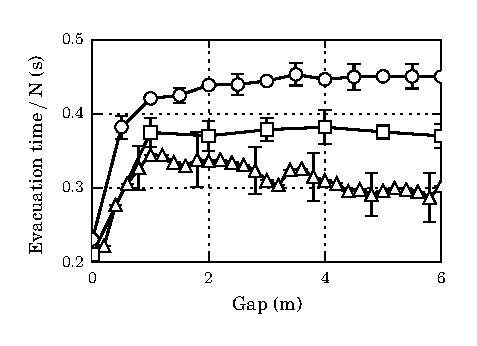
\includegraphics[scale=1]{figuras/fig1_version0.eps}
    \hfill
    \includegraphics[scale=1]{figuras/gap_vste_225_v4_v8.eps}
    \caption[width=5cm]{Izquierda: Gráfico de tiempo de evacuación por individuo vs. gap para recintos de $20\times 20$~(m) (círculos), $30\times 30$~(m) (triángulos) y $40\times 40$~(m) (cuadrados) con 225, 580 y 961 individuos respectivamente. Todos los recintos tienen dos puertas, cada una de ancho $L=1,2$~m. Las gráficas corresponden al promedio de treinta iteraciones. Para todos los casos, la velocidad deseada del individuo fue de $v_d=4$~m/s. Cada simulación termina cuando evacúan 160, 529 y 961 individuos respectivamente.
    Derecha: Gráfico de tiempo de evacuación en función del gap. El recinto es de $20\times 20$~(m) con 225 individuos y dos puertas, cada una tiene un ancho de $L=1,2$~m. La gráfica corresponde al promedio de treinta iteraciones. Las velocidades de deseo de los individuos es de $v_d=4$~m/s (círculos) y $v_d=8$~m/s (cuadrados). Cada simulación termina cuando evacúan 160 individuos.}
    \label{gap_vste_vel_n}
\end{figure}


\subsection{Blocking clusters}

En esta subsección se mostrarán las diferencias en la probabilidad de formar clusters de bloqueo grandes (que abarcan ambas puertas) y chicos (abarcan solo una puerta). También se muestra cómo esta probabilidad depende de la cantidad de individuos y la velocidad de deseo. Recordemos que la probabilidad de formar blocking clusters se define como la razón entre el tiempo que hay blocking clusters constituidos y el tiempo total de simulación. \\

Un sistema de 225 individuos con $v_d=4$~m/s manifiesta, en la figura \ref{proba_vsgap_v4_big_small}, que la probabilidad de formar big blocking clusters (círculos) decae con la separación de las puertas. Es decir, cuanto más lejos están las puertas es más difícil tener un conjunto de individuos que vaya de una pared a otra.
Por otro lado, la probabilidad de formar clusters de bloqueo pequeños (bloqueos de una única puerta) tiene una forma funcional que alcanza el máximo en el $g_c$ y luego desciende. Este descenso se debe a que al estar separadas las puertas disminuye la presión que hay en cada bulk, esto hace que los individuos tengan menos probabilidad de formar blocking clusters. El comportamiento de esta función es similar al de tiempo de evacuación en función del gap (figura \ref{gap_vste_225_v4}).\\

El tamaño del gap crítico equivale al ancho de dos individuos. Este tamaño favorece la formación de dos blocking clusters (uno para cada puerta). Esto genera un aumento de los bloqueos que se manifiesta en un incremento del tiempo de evacuación. 


\begin{figure}[H]
    \centering
    \includegraphics[scale=1.6]{figuras/proba_vsgap_v4_big_small.eps}
    \caption[width=5cm]{Probabilidad de formar ``big" (círculos) y ``small" (cuadrados) blocking clusters (bloqueos de dos y una puerta respectivamente), ambos en función del gap. El recinto es de $20\times 20$~(m) con 225 individuos y dos puertas, cada una tiene un ancho de $L=1,2$~m. Las gráficas corresponden al promedio de treinta iteraciones diferentes. La velocidad de deseo es de $v_d=4$~m/s. Cada simulación termina cuando evacúan 160 individuos.}
    \label{proba_vsgap_v4_big_small}
\end{figure}

La probabilidad de formar clusters de bloqueo está vinculada al número de individuos y la velocidad de deseo. Esto puede verse en la figura \ref{proba_vsgap_all} donde la curva con triángulos representa la probabilidad de formar blocking clusters para un recinto con 961 individuos, la curva que está debajo (cuadrados) es para un sistema con 225 individuos con velocidad de deseo $v_d=6$~m/s y la curva con círculos corresponde a $v_d=4$~m/s y 225 peatones. Incrementar N o $v_d$ produce un aumento de la probabilidad de formar clusters de bloqueo. Es decir, si los individuos tienen alta ansiedad o si el tamaño de la multitud es grande, aumentan los lapsos de tiempo en los cuales las puertas están bloqueadas.  

\begin{figure}[H]
    \centering
    \includegraphics[scale=1.6]{figuras/proba_vsgap_all.eps}
    \caption[width=5cm]{Probabilidad de formar small blocking clusters (bloqueos de una sola puerta) en función del gap, para un recinto $20\times 20$~(m) con 225 individuos a $v_d=4$~m/s (círculos) y $v_d=6$~m/s (cuadrados). Lo mismo para un recinto de $40\times 40$~(m) con 961 individuos a $v_d=4$~m/s (triángulos). Ambos recintos poseen dos puertas, cada una tiene un ancho de $L=1,2$~m. Las gráficas corresponden al promedio de treinta iteraciones diferentes. Las simulación terminan cuando evacúan 160 individuos y 864 respectivamente.}
    \label{proba_vsgap_all}
\end{figure}


\subsection{Presión}

En esta subsección se describirán los diagramas de isobaras para recintos con dos puertas separadas por un gap. 
Cuando la separación es nula (gap cero) se recupera una distribución de presión similar a las distribuciones de la sección anterior. La presión máxima se da en los costados ya que en el medio se forma un canal por donde la gente puede transitar (figura \ref{presion_225p_g0}). Se tiene simetría de reflexión con respecto al eje $y=10$~m. 
\begin{figure}[H]
    \centering
    \includegraphics[scale=1.6]{figuras/press_225p_v4_g0.eps}
    \caption[width=5cm]{Isobaras cercanas a la puerta; la escala a la derecha está expresada en [P]=N/m. La salida está centrada en la posición $x=20$~m e $y=10$~m, son dos puertas de ancho $L=1,2$~m con $g=0$~m. El recinto es de $20\times 20$~(m) con 225 individuos. La gráfica corresponde a valores medios a lo largo de 30 procesos de evacuación. Se usó un grillado de 1m$^2$ para promediar el campo de presiones (P). La velocidad deseada de los individuos fue de $v_d=4$~m/s. Las barras rojas representan las paredes laterales.}
    \label{presion_225p_g0}
\end{figure}

En las figuras de \ref{presion_225p_g1_5_y_5} se muestran isobaras de presión. Cuando la separación entre puertas equivale al gap crítico $g_c=1,5$~m, la zona de más alta presión se extiende en superficie. Si $g=5$~m los focos de máxima presión se separan ya que a esta distancia los bulks están suficientemente lejos como para que las interacciones entre éstos sean chicas. Puede verse que cuando el gap es grande no existen zonas de presión alta ($>$7000 N/m). Separar las puertas una distancia considerable produce una disminución general de la presión. \\

Recordemos que en este trabajo la definición de presión usada es la que se desarrolla en~\cite{Helbing1} y se expresa en la fórmula (\ref{phelbing}).

\begin{figure}[H]
    \centering
    \includegraphics[scale=1]{figuras/isobaras_g1_5.eps}
    \hfill
        \includegraphics[scale=1]{figuras/isobaras_g5.eps}	
    \caption[width=5cm]{Isobaras cercanas a la puerta; la escala a la derecha está expresada en [P]=N/m. La salida consta de dos puertas de ancho $L=1,2$~m separadas entre sí por una distancia de $g=1,5$~m y $g=5$~m (figuras de izquierda y derecha respectivamente), puertas centradas en $x=20$~m e $y=11,35$~m y $x=20$~m e $y=8,65$~m (izquierda) y $x=20$~m e $y=12,5$~m y $x=20$~m e $y=7,5$~m (derecha) . El recinto es de $20\times 20$~(m) con 225 individuos. Las gráficas corresponden a valores medios a lo largo de 30 procesos de evacuación. Se usó un grillado de 1m$^2$ para promediar el campo de presiones (P). La velocidad deseada de los individuos fue de $v_d=4$~m/s. Las barras rojas representan las paredes laterales.}
    \label{presion_225p_g1_5_y_5}
\end{figure}

En esta sección se discutieron los resultados para recintos con dos puertas separadas por una separación o gap. Se obtuvo que el efecto ``faster is slower" vale para distintos grados de separación. Las curvas de tiempo de evacuacón presentan un cambio en la pendiente luego del gap crítico ($g_c$=1,5~m). El comportamiento cualitativo de la probabilidad de formar blocking clusters es similar al del tiempo de evacuación. Por lo tanto el bloqueo de cada una de las puertas es un factor determinante en la evacuación. En cuanto a la presión, si las puertas están suficientemente alejadas se produce una disminución general de la misma ya que los bulks formados cuentan con menos individuos. 

\chapter{Conclusiones}
En este trabajo de tesis se implementaron códigos que permitieron realizar simulaciones de multitudes evacuando en estado de pánico según el modelo de fuerza social. \\

Para recintos con una única salida se obtuvieron dinámicas diferentes según el tamaño de la puerta. Si esta es ancha, el flujo de evacuación es permanente (\emph{i.e.} prácticamente no hay momentos en los que todos los peatones se encuentren sin poder moverse). Las zonas de mayor presión se dan a los costados de la puerta. Cuando la salida es angosta la evacuación es intermitente (\emph{i.e.} por momentos algunos peatones logran salir y en otras ocasiones todos están quietos); este efecto de Stop-and-go hace que la zona de máxima presión se de en el medio del bulk (dos metros antes de la puerta aproximadamente). 
Para ambos recintos la mayor velocidad de los individuos se tiene en el medio. \\

En cuanto a los recintos con dos puertas en un mismo lado, se obtuvo  una separación crítica para la cual cambia la pendiente de la curva tiempo de evacuación vs. separación (gap). Este valor es $g_c=1,5$~m y coincide aproximadamente con el ancho de dos peatones. Esta cantidad es independiente del número de individuos y la velocidad de deseo. Esto permitió afirmar que el $g_c$ afecta a los bloqueos que ocurren en las cercanías de la salida. \\

La forma funcional de la probabilidad de formar small blocking clusters es similar a la forma funcional del tiempo de evacuación, esto denota que los bloqueos de cada una de las puertas son determinantes en la eficiencia de la evacuación. \\

Aumentar el nivel de ansiedad de los individuos mediante la velocidad de deseo genera evacuaciones más lentas así como aumentar la cantidad de individuos en el recinto. Esto coincide con los resultados obtenidos de la presión que soportan los individuos del blocking cluster. En todos los casos aumentar $v_d$ o N genera un incremento de la presión y tiene como consecuencia evacuaciones menos eficientes.\\

El mejor rendimiento en las evacuaciones se dio cuando las puertas no tienen separación entre sí ($g=0$~m). Separar la salida en dos puertas empeora el rendimiento a pesar de que la apertura total tenga el mismo tamaño. Pero, si por razones estructurales hay que construir dos puertas lo mejor es hacerlo dejando una distancia de separación de por lo menos 6~m (bajo las condiciones de estudio de este trabajo).    

\begin{appendices}
\chapter{Presión}
\label{appendix:presion}

Este apéndice está destinado a aclarar el significado de la "presión social" actuando sobre un individuo y la presión colectiva (presión de \textit{bulk}).  
\\
\subsection{\label{social_pressure}La presión social}

La figura ~\ref{hilera2} representa una hilera de individuos empujando a la derecha. La pared impide el movimiento de los peatones. Todos los individuos de la hilera están en su posición de equilibrio $x_1,x_2,...,x_{i},...x_N$, mientras que la pared está en la posición $x_0=0$. 

\begin{figure}[!htbp]
\center
\includegraphics[scale=1]{figuras/hilera.eps}
\caption{\label{hilera2} Hilera de individuos empujando a la derecha. El eje horizontal indica la posición positiva. }
% done with figuras_presion.odg
\end{figure}

Los peatones empujan a la derecha gracias a la fuerza de deseo
$f_d^{(i)}=mv_d/\tau$, según la ecuación Ec.~(\ref{fdeseo}). La repulsión social balancea la fuerza de deseo, pero solo se tiene en cuenta la interacción de los individuos en contacto (se desprecia la interacción de segundos vecinos). La ec ~\ref{eqn_6} muestra la ecuación de balance de cada individuo en la hilera. \\

\begin{equation}
 f_s^{(i,i+1)}-f_s^{(i,i-1)}+\displaystyle\frac{mv_d}{\tau}=0\label{eqn_6}
\end{equation}

\noindent con $f_s^{(i,j)}$ la fuerza repulsiva que siente el individuo $i$ debido a la presencia del peatón $j$. Cabe destacar que la condición de contorno en la posición $x_0=0$  es condición de Dirichlet, mientras que la condición en el otro extremos es condición de Neumann $f_s^{(N,N+1)}=0$. Las fuerzas en los peatones se obtienen de forma recursiva a partir de la expresión Ec.~\ref{eqn_6}, empezando desde el extremo libre ($i=N$). El resultado es

\begin{equation}
f_s^{(i,i-1)}=(N-i+1)\,\displaystyle\frac{mv_d}{\tau}\ \ \ , \ \ \ 
i=1,....,N\label{eqn_7}
\end{equation}

\noindent con las correspondientes posiciones  $x_1,x_2,...,x_{i},...x_N$ obtenidas a partir de la sustitución de la fuerza social expresada en Ec.~\ref{eqn_2}, comenzando en la posición de la pared.

\begin{equation} 
x_i=x_{i-1}-(r_{i}+r_{i-1})+B\,\ln\bigg[(N-i+1)\,\displaystyle\frac{mv_d}{A\tau}
\bigg]\label{eqn_8}
\end{equation}

La intuición sugiere que la presión que siente un peatón $P_i$ 
corresponde a las fuerzas actuando en él (por unidad de área) debido a los primeros vecinos. De la definición de "función de presión social" (\ref{eqn_4}) se puede derivar

\begin{equation}
P_i=\displaystyle\frac{1}{2}\,\bigg[\displaystyle\frac{x_{i}-x_{i+1}}{3V_i}\,
f_s^ { (i , i+1) } +\displaystyle\frac { x_ {i-1}-x_{i}}{3V_i}\,f_s^{(i,i-1) 
}\bigg]\label{eqn_9}
\end{equation}

\vspace{3mm}

\noindent donde la magnitud $x_{ij}/3V_i$ corresponde a la inversa de la superficie efectiva del peatón. Para individuos modelados como esferas rígidas, la distancia entre peatones es $x_{ij}=2r_i$ y el volumen $V_i=4\pi r_i^3/3$. Por lo tanto, 

\begin{equation}
P_i=\displaystyle\frac{1}{4\pi 
r_i^2}\,\bigg[f_s^ { (i , i+1) } +f_s^{(i,i-1)}\bigg]\label{eqn_10}
\end{equation}

\noindent como es de esperar para la presión del individuo.  \\

\subsection{\label{bulk_pressure}La presión de bulk}

Se puede verificar la relación de virial (\ref{eqn_5}) a través de la expresión (\ref{eqn_9}). Agregando los términos de la hilera de $N$ peatones y reemplazando el primer y último término por las correspondientes condiciones de contorno. Esto da como resultado,


\begin{equation}
\left\{\begin{array}{lcl}
3P_1V_1 
& = &\displaystyle\frac{x_{1}}{2}f_s^ { (1 , 2)} - 
\displaystyle\frac{x_{2}}{2}\,f_s^ { (1 , 2) }  \\
&& \\
3P_2V_2 
& = &\displaystyle\frac{x_{2}}{2}\,\big[f_s^ { (2 , 3)} - f_s^{(2,1)} 
\big] - \displaystyle\frac{x_{3}}{2}\,f_s^ { (2 , 3) } +\displaystyle\frac 
{ x_ {1}}{2}\,f_s^{(2,1) 
} \\
&& \\
3P_3V_3 
& = &\displaystyle\frac{x_{3}}{2}\,\big[f_s^ { (3 , 4)} - f_s^{(3,2)} 
\big] - \displaystyle\frac{x_{4}}{2}\,f_s^ { (3 , 4) } +\displaystyle\frac 
{ x_{2}}{2}\,f_s^{(3,2) 
} \\
... &&\\
&& \\
3P_NV_N 
& = &-\displaystyle\frac{x_{N}}{2}\, f_s^{(N,N-1)} 
+\displaystyle\frac{ x_{N-1}}{2}\,f_s^{(N,N-1) 
} \\
 \end{array}\right.\label{eqn_11}
\end{equation}

Estas son las presiones locales en cada peatón debido al contacto entre individuos (excluyendo las paredes). La suma de los términos resulta la ecuación de virial como esta expresada en (\ref{eqn_5})

\begin{equation}
\begin{array}{lcl}
\displaystyle\sum_{i=1}^N 3P_iV_i & = & (x_1 - x_2)f_s^{(1,2)} + (x_2 - 
x_3)f_s^{(2,3)} +... \\
& + &  (x_{N-1}-x_N)f_s^{(N,N-1)} \\
&& \\
& = & x_{1}\,\displaystyle\frac{N\,mv_d}{\tau} - 
\displaystyle\sum_{i=1}^N x_i\,\displaystyle\frac{mv_d}{\tau} \\
 \end{array}\label{eqn_12}
\end{equation}

\noindent donde el primer término corresponde a la presión global
$-3\mathcal{PV}$. Notar que $x_1$ es negativo, y $3\mathcal{PV}$ es definido positivo. El último término también es positivo, le agrega presión al bulk debido a las fuerzas de deseo.  
\\
La relación de virial (\ref{eqn_5}) permite calcular la presión de \textit{bulk} en un grupo de peatones. Por ejemplo, la presión en los  $M$ peatones más cercanos a la pared corresponde a la fuerza actuando en este grupo debido a los $N-M$ restantes. Según la Ec.~(\ref{eqn_5}), la presión en los $M$ individuos es


\begin{equation}
 \displaystyle\sum_{i=1}^M 3P_iV_i 
=-3\mathcal{PV}-\displaystyle\sum_{i=M+1}^N 3P_iV_i-\displaystyle\sum_{i=1}^N 
x_i\displaystyle\frac{mv_d}{\tau}\label{eqn_13}
\end{equation}

La presión de bulk en los primeros $M$ individuos aumenta con la cantidad de peatones incluidos en la multitud. Esto se verifica evaluando las ecuaciones~(\ref{eqn_12}) y (\ref{eqn_13}) incrementando el valor de $N$.\\

Las Ecs~(\ref{eqn_7}) y (\ref{eqn_8}) permiten calcular el perfil de presiones en función de la distancia a la pared. El perfil es similar al medido en un proceso de evacuación.

La figura~\ref{fig:10} representa un histograma de la presión en cada peatón. \\

\begin{figure}[H]
    \centering
    \includegraphics[scale=0.8]{figuras/p_dist.eps}
    \caption[width=5cm]{Presión media en función de la distancia a la salida. El tamaño del recinto fue $20\,\mathrm{m}\times20\,\mathrm{m}$  con una puerta de $L=1.2$~m width. Los valores medios fueron calculados a partir de 30 procesos hasta que 100 peatones abandonaron la habitación. La velocidad de deseo fue $v_d=4\,$m/s. La distancia a la puerta fue dividida en bins de tamaño $0.3$~m o 1~m.  El símbolo $\bigcirc$  corresponde a bins de $0.3$~m. El símbolo $\bigtriangleup$ corresponde a bins de 1~m, pero en este caso los datos corresponden a  $9.5\,\mathrm{m}\leq y\leq 10.5\,\mathrm{m}$ }
    \label{fis_g}
\end{figure}




\chapter{Script básico de Lammps}
\label{appendix:script}

A modo de ejemplo se describirá un script de Lammps que se hizo para simular 225 individuos en un recinto de 20$\times$20~m con una puerta de 1,2~m. Este programa cuenta con dos ciclos {\tt for}, uno recorre diferentes valores de velocidad de deseo y el otro (anidado) sirve para tener 30 simulaciones con diferentes velocidades iniciales. \\

El programa devuelve un video de la simulación en formato mpg y un archivo txt con una tabla que indica: $v_d$, número de iteración y el tiempo para el cual evacuaron más de 159 individuos.
El script está dividido en cinco partes: condiciones iniciales, fuerzas, evacuados, visualización y ejecución del proceso.\\ 

En las condiciones iniciales se fija la dimensión del problema (2d), las condiciones de contorno (no periódicas en las coordenadas x e y), el sistema de unidades usado (sistema internacional), también se configuran los atributos de los individuos como el tamaño (60 cm diámetro) y su peso (70~kg). La velocidad inicial se fijó con la función {\tt velocity}, la misma genera una distribución gausiana de velocidades que es asignada de forma aleatoria a los individuos. El módulo de la velocidad es 1,7~m/s. La semilla que genera la distribución de velocidades es el número de iteración.\\

En cuanto al tamaño de la región de simulación, se crearon tres zonas: la zona 1 es la que inicialmente posee a los individuos (ordenados tipo red cuadrada separados 1,3~m entre si), la zona 2 es la región de evacuación y la zona 3 es la conexión entre ambas regiones (la puerta por donde pasan).\\

En la parte de fuerzas se especifican las interacciones que sienten los individuos y sus respectivos parámetros. La repulsión entre individuos (pair style social) utiliza la expresión ($\ref{fsocial}$) con los parámetros: A=2000~N, B=0,08~m y se asignó un cutoff de 3,5~m. La fuerza granular (pair style gran/social) se basa en la fórmula ($\ref{frozamiento}$) con $\kappa =2,4 \times 10^5$~kgm$^{-1}$s$^{-1}$. Se usaron los mismos parámetros para las expresiones análogas en la interacción individuo-pared (fix wall/region social y granular). La fuerza de deseo (fix social/self) tomó como parámetro a la velocidad de deseo, ésta varía según el loop del encabezado del programa. \\

En la parte de evacuación se cuenta a todos los individuos que salieron del recinto, es decir, a todos los peatones cuya posición en la coordenada x sea mayor a 20 m. Este cálculo queda almacenado en la variable {\tt evacuados} que se utiliza para terminar la simulación cuando la cantidad de individuos evacuados sea superior a 159. \\
La visualización devuelve un video {\tt in.evacuation.mpg} que permite observar la dinámica de la evacuación. \\

La última parte del programa está destinada a la ejecución del proceso. Calcula nuevas posiciones y velocidades usando el algoritmo de Verlet a través de la función {\tt fix nve}. El timestep utilizado es 0,0001 s. La función {\tt run} 500 aplica 500 iteraciones de Verlet. En la variable {\tt t} se calcula y guarda el tiempo. Una vez que se supera la cantidad de individuos requerida, la función {\tt print} escribe en un txt las siguientes variables: velocidad de deseo, número de iteración y tiempo de evacuación (el tiempo que tardan evacuar más de 159 peatones).\\

En la sintaxis de Lammps, todo texto seguido de un numeral es comentario. A continuación se muestra el código arriba descripto.

\begin{verbatim}
## 2D Panic Evacuation: 225 individuals, room 20x20
#	Loop velocidad de deseo
variable vdmax equal 6
variable vd loop 1 ${vdmax}
label start_of_loop1
#	Loop de iteracion
variable itermax equal 30
variable iter loop 1 ${itermax}
label start_of_loop2

#           INITIAL CONDITIONS
dimension        2
boundary         f f p
units            si
atom_style       sphere
lattice          sq 1.3 origin 0.5 0.5 0.0
region           zona1 block 0 20 0 20 -1 1 units box
region           zona2 block 20.12 40 0 20 -1 1 units box
region           zona3 block 19 21 9.4 10.6 -1 1 units box
region           todas union 3 zona1 zona2 zona3
create_box       1 todas
create_atoms     1 region zona1
set              atom * mass 70.0
set              atom * diameter 0.6
velocity         all create 1e23 ${iter} dist gaussian
comm_modify      vel yes

#           FORCES
pair_style  hybrid/overlay gran/social 0 0 0 240000 0 1 social 0.08 3.5
pair_coeff  * * social 2000 3.5 0.3
pair_coeff  * * gran/social
fix  walls  all wall/region todas social 2000 0.08 3.5
fix  wallg  all wall/region todas granular 240000 120000 0.001    
fix  target all social/self 70 ${vd} xy          

#           EVACUATED
compute     1 all property/atom x
variable    out atom c_1>20.0
compute     mycompute all reduce sum v_out
variable    evacuados equal c_mycompute

#           VISUALIZE
dump  3 all movie 200 in.evacuation.mpg type type &
      axes yes 0.8 0.02 view 0 0 zoom 2 adiam 0.6

#           RUN THE PROCESS
atom_modify   sort 0 0.0
timestep      0.0001
fix           1 all nve
thermo_style  custom step c_mycompute

#	Loop de proceso
variable  nmax equal 20000
variable  n loop ${nmax}
label     start_of_loop3
run       500
if        "${evacuados} > 159" then "jump SELF break"
variable  t equal 0.05*$n
next n
jump SELF start_of_loop3
#	Terminación del proceso
label break
print "${vd}  ${iter}  $t" append print.txt
clear
variable n delete
next iter
jump SELF start_of_loop2
#	Terminacion loop de itercion
clear
next vd
jump SELF start_of_loop1
#	Terminación loop velocidad de deseo
\end{verbatim}

\chapter{Caracterísicas del cluster}
\label{caracteristicas_tecnicas}

En este apéndice se detallan las características de las computadoras utilizadas para llevar a cabo las simulaciones. Se usaron dos computadoras. Una de ellas compuesta por cuatro nodos (Head, node1, node2, node3) y otra por un único nodo. 

\begin{verbatim}

Head

Architecture:          x86_64
CPU op-mode(s):        32-bit, 64-bit
Byte Order:            Little Endian
CPU(s):                2
On-line CPU(s) list:   0,1
Thread(s) per core:    1
Core(s) per socket:    2
Socket(s):             1
NUMA node(s):          1
Vendor ID:             GenuineIntel
CPU family:            15
Model:                 6
Model name:            Intel(R) Pentium(R) D CPU 3.20GHz
Stepping:              4
CPU MHz:               2400.000
BogoMIPS:              6400.33
Virtualization:        VT-x
L1d cache:             16K
L2 cache:              2048K
NUMA node0 CPU(s):     0,1

Node1:

Architecture:          x86_64
CPU op-mode(s):        32-bit, 64-bit
Byte Order:            Little Endian
CPU(s):                8
On-line CPU(s) list:   0-7
Thread(s) per core:    2
Core(s) per socket:    4
Socket(s):             1
NUMA node(s):          1
Vendor ID:             GenuineIntel
CPU family:            6
Model:                 42
Model name:            Intel(R) Core(TM) i7-2600 CPU @ 3.40GHz
Stepping:              7
CPU MHz:               2897.703
BogoMIPS:              6784.38
Virtualization:        VT-x
L1d cache:             32K
L1i cache:             32K
L2 cache:              256K
L3 cache:              8192K
NUMA node0 CPU(s):     0-7


Node 2:

Architecture:          x86_64
CPU op-mode(s):        32-bit, 64-bit
Byte Order:            Little Endian
CPU(s):                8
On-line CPU(s) list:   0-7
Thread(s) per core:    2
Core(s) per socket:    4
Socket(s):             1
NUMA node(s):          1
Vendor ID:             GenuineIntel
CPU family:            6
Model:                 60
Model name:            Intel(R) Core(TM) i7-4790 CPU @ 3.60GHz
Stepping:              3
CPU MHz:               3990.234
BogoMIPS:              7200.41
Virtualization:        VT-x
L1d cache:             32K
L1i cache:             32K
L2 cache:              256K
L3 cache:              8192K
NUMA node0 CPU(s):     0-7


Node3:

Architecture:          x86_64
CPU op-mode(s):        32-bit, 64-bit
Byte Order:            Little Endian
CPU(s):                4
On-line CPU(s) list:   0-3
Thread(s) per core:    1
Core(s) per socket:    4
Socket(s):             1
NUMA node(s):          1
Vendor ID:             GenuineIntel
CPU family:            6
Model:                 42
Model name:            Intel(R) Core(TM) i5-2500 CPU @ 3.30GHz
Stepping:              7
CPU MHz:               2758.851
BogoMIPS:              6584.92
Virtualization:        VT-x
L1d cache:             32K
L1i cache:             32K
L2 cache:              256K
L3 cache:              6144K
NUMA node0 CPU(s):     0-3


\end{verbatim}


\begin{verbatim}

Architecture:          x86_64
CPU op-mode(s):        32-bit, 64-bit
Byte Order:            Little Endian
CPU(s):                8
On-line CPU(s) list:   0-7
Thread(s) per core:    2
Core(s) per socket:    4
Socket(s):             1
NUMA node(s):          1
Vendor ID:             GenuineIntel
CPU family:            6
Model:                 58
Stepping:              9
CPU MHz:               1600.000
BogoMIPS:              6784.26
Virtualization:        VT-x
L1d cache:             32K
L1i cache:             32K
L2 cache:              256K
L3 cache:              8192K
NUMA node0 CPU(s):     0-7

\end{verbatim}
\end{appendices}
\bibliographystyle{plain} %Choose a bibliograhpic style
\bibliography{bibliografia/biblio}



\end{document}